\lez{23}{15-04-2020}{}
\subsection{Generalità sui fononi}%
\label{sub:Generalità sui fononi}
In generale i fononi nei cristalli sorgono risolvendo l'equazione secolare:
\[
    \ddot{u}_i\left( \v{R}_I \right) 
    =
    \v{D}_{ij,IJ}u_j(\v{R}_I) 
.\] 
Dove $u_i( R_I )$ è lo spostamento dell'atomo i-esimo dalla posizione di equilibrio nel sito $R_I$ del reticolo, mentre $\v{D}$ è la matrice dinamica: la matrice delle derivate seconde dell'energia nelle posizioni di equilibrio ( Hessiano ).\\
Assumendo che le soluzioni a tale equazione siano onde piane:
\[
    u_i( \v{R}_I ) = \mathcal{E}_i e^{i( \v{q}\cdot\v{R}-\omega t ) }
.\] 
otteniamo la forma standard per l'equazione secolare:
\[
    \omega^2\mathcal{E}_i=\v{D}_{ij}( \v{q} ) \mathcal{E}_j 
.\] 
Questa equazione ha 3 soluzioni per ogni valore di $\v{q}$. Inoltre la simmetria del cristallo assicura che tali soluzioni sono funzioni di Bloch, quindi i 3 autovalori $\omega_I(\v{q})$ possono essere valutati all'interno della prima zona di Brillouin.\\
Notiamo che se nella cella unitaria sono presenti $N$ atomi allora le soluzioni a tale equazione sono $3N$.\\
\subsection{Struttura del Silicio e del carburo di Silicio.}%
\label{sub:Struttura del Silicio e del carburo di Silicio.}
Entrambe queste strutture hanno una cella di tipo ZB: FCC con due atomi per base. 
\begin{figure}[ht]
    \centering
    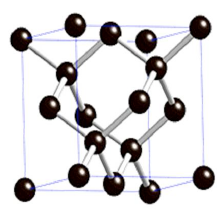
\includegraphics[width=0.2\textwidth]{figures/Si-struttura.png}
    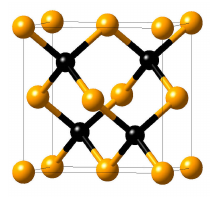
\includegraphics[width=0.2\textwidth]{figures/SiC-struttura.png}
    \caption{Struttura di un cristallo di Silicio (sinistra) e di un cristallo di carburo di Silicio (destra), le due figure mostrano la stessa struttura sotto diverse prospettive.}
    \label{fig:-figures-SIC-SI-struttura}
\end{figure}
Entrambe le strutture hanno 3 rami ottici e 3 rami acustici per la propagazione di fononi con differenti polarizzazioni:
\begin{itemize}
    \item Una longitudinale.
    \item Due trasverse.
\end{itemize}
Generalmente le onde longitudinali hanno energia maggiore delle trasverse (per i modi acustici questo è sempre vero). I rami trasversi tendono inoltre ad essere degeneri.\\
Esistono dei punti di simmetria in questi cristalli, in tali punti si ha la degenerazione dei rami fononici (nel loro $k$ corrispondente nel reticolo reciproco). Gli andamenti dei rami sono i seguenti:
\begin{figure}[H]
    \centering
    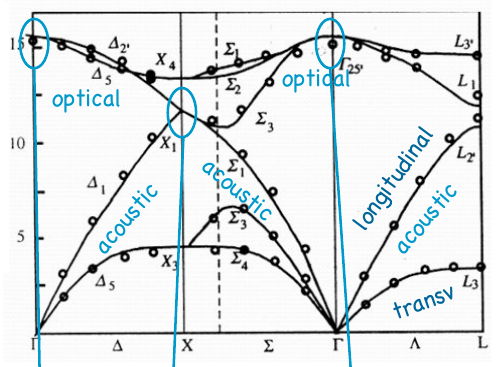
\includegraphics[width=0.4\textwidth]{figures/Si-rami.png}
    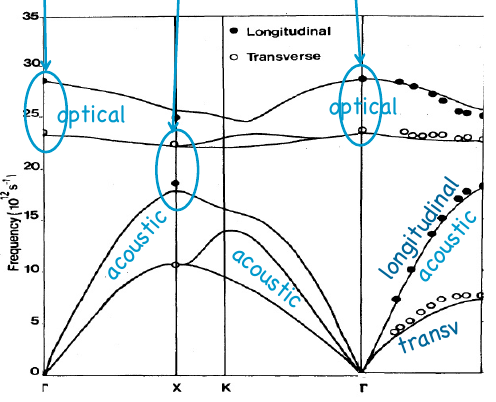
\includegraphics[width=0.4\textwidth]{figures/SiC-rami.png}
    \caption{Rami dei fononi per il Silicio (sinistra) e per il carburo di Silicio (destra).}
    \label{fig:figures-SiC-rami-png}
\end{figure}
Se assumiamo che $q<(1/5)(\pi /a)$ (quindi $\lambda >10a$) i grafici nella Figura \ref{fig:figures-SiC-rami-png} sono nel regime lineare (confinati intorno alla origine) e che ovviamente vediamo solo i rami acustici. In questa zona notiamo che fononi longitudinali e trasversi hanno diverse velocità di propagazione e che i due modi trasversi tendono a degenerare. 
\subsection{Onde longitudinali nei liquidi e nei gas}%
\label{sub:Onde longitudinali nei liquidi e nei gas}
Dimostriamo che qualunque sistema avente una compressibilità finita può sostenere il trasporto di onde longitudinali. \\
Prendiamo l'equazione di newton e di continuità:
\[\begin{aligned}
    &\frac{\partial P}{\partial x} + \rho\frac{\partial v}{\partial t} = 0\\
    &\frac{\partial \rho}{\partial t} + \frac{\partial }{\partial x} (\rho v) = 0 
.\end{aligned}\]
Prendiamo una perturbazione della densità (pressione) per linearizzare l'equazione:
\[\begin{aligned}
    &P=P_0+P'\\
    &\rho =\rho_0+\rho'\\
    &v=v'
.\end{aligned}\]
Inserendo queste perturbazioni:
\[\begin{aligned}
    &\frac{\partial P'}{\partial x} + \rho_0 \frac{\partial v'}{\partial t} = 0\\
    &\frac{\partial \rho'}{\partial t} + \rho_0 \frac{\partial v'}{\partial x} = 0
.\end{aligned}\]
Per risolvere dobbiamo introdurre una equazione di stato:
\[\begin{aligned}
    &\rho =\rho (P_0) + \frac{\partial \rho}{\partial P} P'\\
    &c^2=\frac{\partial P}{\partial \rho} = \frac{1}{K\rho}
.\end{aligned}\]
Mettendo a sistema si riesce ad ottenere una equazione di D'alambert:
\[
    \frac{\partial ^2\rho'}{\partial x^2}-\frac{1}{c^2}\frac{\partial ^2\rho'}{\partial t^2}  = 0
.\] 
Quindi si hanno onde di densità (longitudinali) come si voleva dimostrare.
\subsection{Teoria della elasticità: legge di Hooke}%
\label{sub:Teoria della elasticità: legge di Hooke}
La legge di Hooke è:
\[
\v{T}=\v{C}\cdot \v{e}
.\] 
Dove si ha che 
\begin{itemize}
    \item $\v{T}=T_{ij}$ è il tensore degli stress, si ha che $\v{F}=\v{T}\hat{n}$.
    \item $\v{e}=e_{ij}=\frac{\partial u_{ij}}{\partial x_j}$ è il tensore degli stress.
    \item $\v{C}=C_{ijkl}$ è il tensore delle costanti elastiche.
\end{itemize}
L'equazione di Newton per un volumetto di materia è:
\[
    \rho dxds\frac{\partial ^2\v{u}}{\partial t^2} = ds\left[\v{f}(x+dx) - \v{f}(x) \right] = dsdx \v{C}\cdot \nabla \v{e} 
.\] 
Che ci porta alla equazione per le onde elastiche nei solidi:
\[
    \rho\frac{\partial ^2 u_i }{\partial t^2}= C_{ikjl}\frac{\partial ^2 u_j}{\partial x_k \partial x_l}  
.\] 
Inoltre possiamo anche notare che la relazione con la matrice dinamica: $\v{D}$ è quadratica in $\v{q}$, per questo motivo abbiamo anche che $\omega$ lineare in $\v{q}$.
\[
D_{ij}= \frac{q_k q_l}{\rho}C_{ikjl}
.\] 
Le soluzioni sono quindi onde non dispersive le cui velocità al quadrato sono combinazioni lineari dei coefficienti $C_{ijkl} /\rho$ e possono essere ricavate risolvendo il problema agli autovalori.\\
Quando il cristallo raggiunge l'equilibrio traslazionale e rotazionale si ha una notevole riduzione delle costanti indipendenti all'interno della matrice delle costanti elastiche $C_{ijkl}$, se inoltre il cristallo ha la forma cubica allora le costanti indipendenti si riducono a 6. In questo modo il calcolo delle velocità di propagazione si semplifica notevolmente.
\subsection{Funzione di risposta e teorema di fluttuazione dissipazione.}%
\label{sub:Funzione di risposta e teorema di fluttuazione dissipazione.}
Definiamo la funzione di risposta di un generico sistema nel seguente modo:
\[\begin{aligned}
    \delta\rho (\v{r}, t) =&
    \int d\v{r}\int_{-\infty}^{t}\chi_l(\v{r}-\v{r}',t-t')v(\v{t}',t')dt=\\ 
    =&
    \int d\v{r}'\int_{-\infty}^{\infty}\chi(\v{r}-\v{r}', t-t') v(\v{r}',t')dt
.\end{aligned}\]
IN cui si fa uso di una funzione di Eavyside per espandere gli estremi di integrazione:
\[
    \chi(\v{r}-\v{r}', t-t') =\chi_l(\v{r}-\v{r}',t-t')\Theta (t-t') 
.\] 
Quindi la funzione $\chi$ è definita per ogni tempo ed è nulla per tempi negativi, a differenza di $\chi_l$ che è definita soltanto per tempi positivi. Andando in trasformata di Fourier si ha che le convoluzioni diventano prodotti:
\[
    \delta\overline{\rho}(\v{k},\omega) 
    = \overline{\chi}(\v{k},\omega) \overline{v}(\v{k},\omega) 
.\] 
Mentre la trasformata spazio-temporale della $\chi$ è:
\[\begin{aligned}
    \overline{\chi}(\v{k},\omega) =&
    	\int d\omega' \overline{\chi}_l(\v{k},\omega-\omega')\Theta (\omega')=\\
    =&
	\int d\omega' \overline{\chi}_l(\v{k},\omega-\omega')
	\left[\frac{1}{2}\delta (\omega') + \frac{i}{2\pi\omega'}\right]=\\
    =&
    	\frac{1}{2}\left[\overline{\chi}_l(\v{k},\omega) + 
    	\int d\omega' \frac{i}{\pi\omega'} 
	\overline{\chi}_l(\v{k},\omega-\omega') \right]
.\end{aligned}\]
$\chi_l$ è reale nel dominio positivo, nel dominio negativo invece può assumere ogni valore. Noi consideriamo il caso in cui $ \overline{\chi}_l(\v{k},\omega)$ sia simmetrico e reale, in tal caso:
\[\begin{aligned}
    &Re\left[ \overline{\chi}(\v{k},\omega)\right] =
    \frac{1}{2}\overline{\chi}_l(\v{k},\omega) \\
    &Im\left[ \overline{\chi}(\v{k},\omega)\right] =
    \frac{1}{2}\int d\omega' 
    \frac{\overline{\chi}_l(\v{k},\omega-\omega')}{\pi\omega'}
.\end{aligned}\]
Questo ci porta ad una prima importante relazione:
\[
    Im\left[\overline{\chi}(\v{k},\omega)\right]=
    \int d\omega' 
    \frac{Re\left[\overline{\chi}(\v{k},\omega-\omega')\right]}{\pi\omega'}
.\] 
Assumendo anche una estensione antisimmetrica di $\chi_l$ abbiamo che $ \overline{\chi}_l(\v{k},\omega)$ è immaginaria (e sempre antisimmetrica).
\[
    Re\left[ \overline{\chi}(\v{k},\omega)\right] =
    -\frac{1}{2}\int d\omega' 
    \frac{\overline{\chi}_l(\v{k},\omega-\omega')}{\pi\omega'}
.\] 
\[
    Im\left[ \overline{\chi}(\v{k},\omega)\right] =
    \frac{1}{2}\overline{\chi}_l(\v{k},\omega) \\
.\] 
Abbiamo quindi le relazioni di Kramers Kronig che nella forma complessa generale si scrivono come:
\[
    \overline{\chi}(\v{k},\omega) = \int \frac{d\omega'}{i\pi}
    \frac{\overline{\chi}(\v{k},\omega)}{(\omega-\omega')}
.\] 
Tali relazioni dipendono dalla causalità del sistema e sono dette trasformate di Hilbert. Matematicamente queste sono collegate da una convoluzione con la funzione di risposta ed una funzione di Heavyside (visto a metodi 2). \\
Notiamo anche che la FT di $ \overline{\chi}$ è indefinita, è definita soltanto la sua trasformata di Laplace e coincide con la FT di $\chi$.\\
Assumiamo adesso che il nostro sistema abbia una perturbazione indipendente dal tempo nella Hamiltoniana:
\[
    H= H_0 - \int d\v{r} v(\v{r}') \delta  \hat{\rho}(\v{r}') 
.\] 
Dove $ \hat{\rho}(\v{r}) = \sum_{}^{} \delta (\v{r}-\v{r}_i)$. Calcolando la media delle fluttuazioni del sistema (classicamente) si ha che:
\[\begin{aligned}
    \delta\rho (\v{r}) =& \left<\delta  \hat{\rho}(\v{r}) \right> =\\
    =&
    \frac{1}{Z}\int \delta  \hat{\rho}(\v{r}) \exp(-\beta H) = \\
    \approx &
    \frac{1}{Z}\int \delta  \hat{\rho}(\v{r}) \exp(-\beta  H_0)
    \left[1+\beta\int d\v{r}'v(\v{r}') \delta  \hat{\rho}(\v{r}')\right]=\\
    =&
    \beta\int d\v{r}'v(\v{r}')
    \left<\delta  \hat{\rho}(\v{r}) \delta\hat{\rho}(\v{r}') \right>_0
.\end{aligned}\]
Quindi otteniamo che:
\[
    \chi_s(\v{r}-\v{r}') 
    = \frac{1}{kT}\left<\delta\hat{\rho}(\v{r})\delta\hat{\rho}(\v{r}')\right>_0
.\] 
La funzione di risposta lineare del sistema ad un campo esterno è collegata alle fluttuazioni spaziali del sistema in assenza di campo esterno (inperturbato)!\\
Usando inoltre la definizione di $S(k)$ (fattore di struttura statica) e la sua relazione con $S(k,\omega)$ possiamo scrivere le seguenti relazioni:
\[\begin{aligned}
    \frac{1}{kT}\left<\left|\rho (\v{k}) \right|^2\right> = &
    \frac{S(k)}{\rho kT} =\\
    =&
    Re\left[\overline{\chi}(\v{k},0)\right] =\\
    =&
    \int \frac{d\omega'}{\pi} 
    \frac{Im\left[\overline{\chi}(\v{k},\omega)\right]}{\omega'} =\\
    =&
    \int d\omega' \frac{S(\v{k},\omega)}{\rho  kT}
.\end{aligned}\]
Nel caso in cui la perturbazione abbia dipendenza temporale si procede in modo analogo sviluppando l'Hamiltoniana, in tal caso si può ottenere:
\[
    \frac{1}{kT}\left<\rho_k(\omega) \rho_{-k}(-\omega)\right> 
    =
    \frac{2}{\omega}Im\left[\overline{\chi}(\v{k},\omega)\right]
.\] 
Questa è la forma del teorema relativa alla dissipazione. La parte immaginaria della funzione di risposta sappiamo infatti essere legata a quest'ultima.\\
Abbiamo ottenuto la forma classica del teorema di fluttuazione dissipazione, nel caso quantistico si può dimostrare che:
\begin{figure}[H]
    \centering
    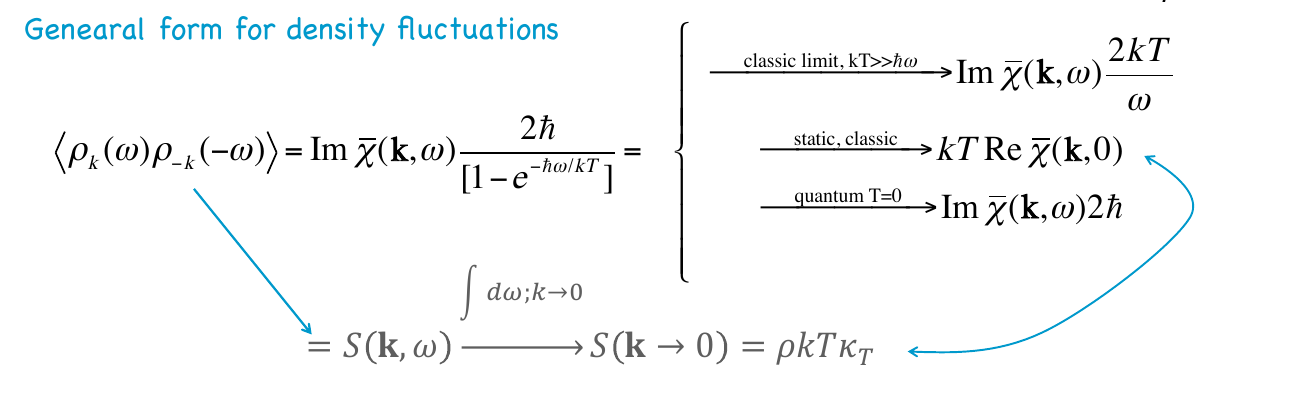
\includegraphics[width=0.9\textwidth]{figures/FluttuDiss-quantistico.png}
    \label{fig:figures-FluttuDiss-quantistico-png}
\end{figure}
Finisce sulle slide della Professoressa Tozzini.
